\chapter{Расчет излучения источников}\label{radiation}
FAINA позволяет рассчитывать электромагнитное излучение от источников с заданными функциями распределения излучающих частиц и другими параметрами. Построены модели следующих типов излучения: синхротронного, обратного комптоновского рассеяния, пионного распада в результате свободно-свободного взаимодействия протонов и тормозного излучения.

\section{Функции распределения частиц}

Важнейшими исходными данными для расчета любого типа излучения является функция распределения излучающих частиц. В коде FAINA для представления распределений используется абстрактный класс ParticleDistribution и семейство наседованных от него классов, соответствующих различным конкретным реализациям. Класс ParticleDistribution имеет следующие доступные методы, описанные в Таблице \ref{ParticleDistribution}:

	\begin{table}
	\begin{center}
		\caption{Публичные методы класса ParticleDistribution }
		\label{ParticleDistribution}
		\begin{small}
		\begin{tabularx}{\textwidth}{|X|X|}
			\hline
			\textbf{ParticleDistribution} & Абстрактный класс для любых распределений частиц\\
			\hline
			distribution(const double\& energy, const double\& mu, const double\& phi) & возвращает функцию распределения от энергии, косинуса полярного угла и азимутального угла, нормированную на единицу \\
			\hline
			virtual distributionNormalized(const double\& energy, const double\& mu, const double\& phi) & чисто виртуальный метод, возвращает функцию распределения от энергии, косинуса полярного угла и азимутального угла, нормированную на концентрацию \\
			\hline
			getConcentration() & возвращает концентрацию частиц\\
			\hline
		\end{tabularx}
	    \end{small}
	\end{center}
\end{table}

Для вычисления излучения необходимо в первую очередь задать распределение излучающих частиц. Для это нужно создать объект из подходящего класса-наследника ParticleDistribution. Дерево наследования на две большие ветви - распределения фотонов, представленных абстрактным классом PhotonDistribution и распределения массивных частиц - MassiveParticleDistribution. Схема наследования этих классов представлена на рисунке \ref{particleDistribution0}. 

\begin{figure}
	\centering
	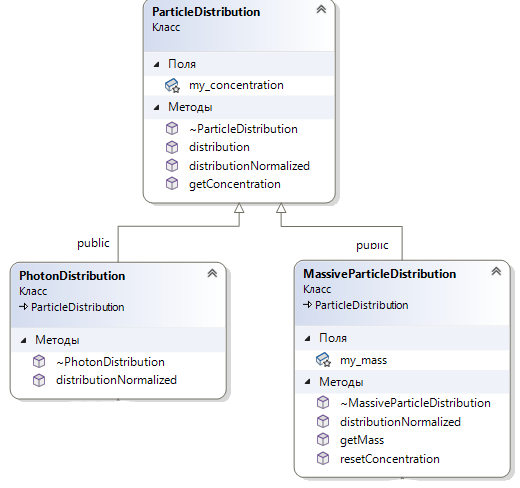
\includegraphics[width=9.5 cm]{./fig/particleDistribution0.png} 
	\caption{Схема наследования распределения фотонов и массивных частиц}
	\label{particleDistribution0}
\end{figure}

Важно отметить, что распределения фотонов не используются для представления результатов расчета излучения. Они нужны как входной параметр для расчета обратного комптоновского рассеяния. Класс PhotonDistribution не имеет дополнительных собственных методов и является лишь интерфейсом. Класс MassiveParticleDistribution тоже является абстрактным, в нем не задан конкретный вид распределения, но добавлены новые методы, описанные в Таблице \ref{MassiveParticleDistribution}	
\begin{table}
	\begin{center}
		\caption{Публичные методы класса MassiveParticleDistribution }
		\label{MassiveParticleDistribution}
		\begin{small}
			\begin{tabularx}{\textwidth}{|X|X|}
				\hline
				\textbf{MassiveParticleDistribution} & Абстрактный класс для распределений массивных излучающих частиц\\
				\hline
				getMass() & возвращает массу частиц \\
				\hline
				resetConcentration(const double\& n) & позволяет изменить полную концентрацию частиц в распределении\\
				\hline
			\end{tabularx}
		\end{small}
	\end{center}
\end{table}
\subsection{Распределения фотонов}

От абстрактного класса PhotonDistribution наследуются следующие классы: абстрактный PhotonIsotropicDistribution, предназначенный для представления изотропных распределений фотонов и CompoundPhotonDistribution, представляющий из себя сумму нескольких распределений фотонов общего вида. Схема наследования классов фотонных распределений представлена на рисунке \ref{photonDistribution}.

\begin{figure}
	\centering
	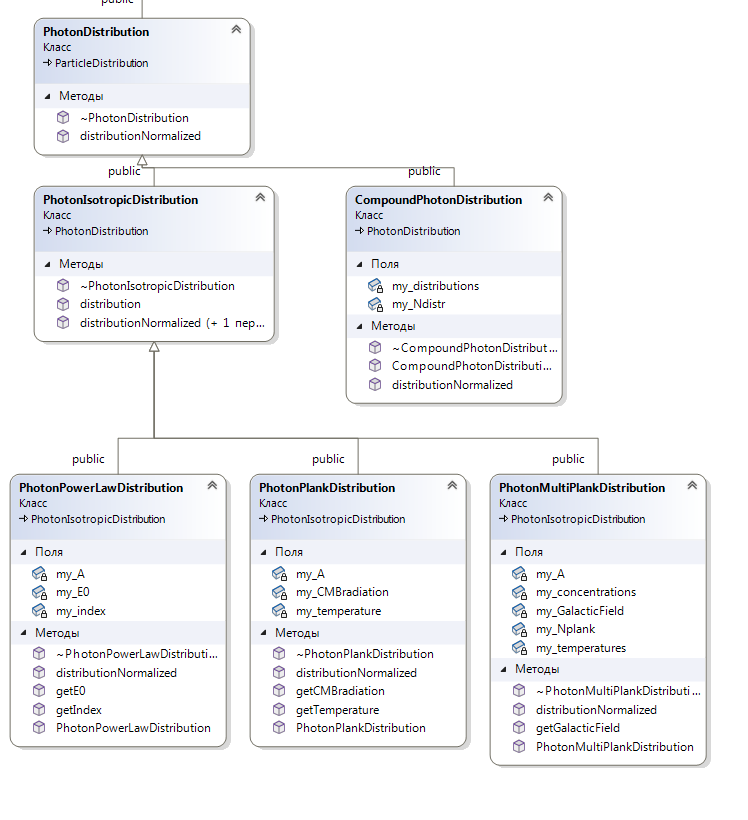
\includegraphics[width=10.5 cm]{./fig/photonDistribution1.png} 
	\caption{Схема наследования классов распределений фотонов}
	\label{photonDistribution}
\end{figure}

У изотропного распределения PhotonIsotropicDistribution добавляются методы, возвращающие значение функции распределения только в зависимости от энергии. Важно понимать, что это не функция распределения по энергии, а полная функция распределения с отброшенными угловыми аргументами. Другими словами, для получения значения функции распределения по энергии нужно домножить значение, возвращенное данным методом на $4 \pi$.

У класса PhotonIsotropicDistribution есть три наследника, которые уже не абстрактные классы, а непосредственно предназначены для создания распределений. Это PhotonPowerLawDistribution для представления степенных распределений, PhotonPlankDistribution, для планковских распределений и PhotonMultiPlankDistribution, для суммы планковских распределений. Метода класса PhotonIsotropicDistribution и его наследников перечислены в таблице \ref{photonDistributionMethods}

\begin{table}
	\begin{center}
		\caption{Публичные методы классов изотропных распределений фотонов}
		\label{photonDistributionMethods}
		\begin{small}
			\begin{tabularx}{\textwidth}{|X|X|}
				\hline
				\textbf{PhotonIsotropicDistribution} & Абстрактный класс для изотропных распределений фотонов\\
				\hline
				distribution(const double\& energy) & возвращает функцию распределения с отброшенными угловыми аргументами, то есть нормированную на концентрацию, деленную на $4 \pi$ \\
				\hline
				virtual distributionNormalized(const double\& energy) & чисто виртуальный метод, возвращает функцию распределения с отброшенными угловыми аргументами, нормированную на  $ 1 / 4 \pi$\\
				\hline
				\textbf{PhotonPowerLawDistribution} & Класс для степенного распределения фотонов\\
				\hline
				PhotonPowerLawDistribution(const double\& index, const double\& E0, const double\& concentration) & конструктор, создающий экземпляр с заданными показателем наклона, начальной энергией и полной концентрацией \\
				\hline
				getIndex() & возвращает показатель наклона спектра\\
				\hline
				getE0() & возвращает минимальную энергию степенного распределения\\
				\hline
				\textbf{PhotonPlankDistribution} & Класс для планковского распределения фотонов\\
				\hline
				PhotonPlankDistribution(const double\& temperature, const double\& amplitude) & конструктор, создающий экземпляр с заданными температурой и апмплитудой - то есть отношением концентрации к равновесному планковскому распределению с данной температурой\\
				\hline
				static getCMBRadiation() & статический метод, возвращающий экземпляр, соответствующий реликтовому излучению (температура $2.725 K$, амплитуда $1$)\\
				\hline
				getTemperature() & возвращает температуру распределения\\
				\hline
				\textbf{PhotonMultiPlankDistribution} & Класс для распределения фотонов, состоящего из суммы планковских распределений\\
				\hline
				PhotonMultiPlankDistribution(int Nplank, const double* const temperatures, const double* const amplitudes) & конструктор, количество планковских распределений, участвующих в смеси, массив их температур и массив амплитуд\\
				\hline
				static getGalacticField() & статический метод, возвращающий экземпляр, соответствующий среднегалактическому фотонному распределению, по данным статьи \cite{Mathis1983}. Данное распределение состоит из пяти планковских компонент, с температурами $2.725K, 20K, 3000K, 4000K, 7000K$ и амплитудами $1.0, 4\cdot10^{4}, 4\cdot10^{-13}, 1.65\cdot10^{-13}, 1.0\cdot10^{-14}$ соответственно\\
				\hline
			\end{tabularx}
		\end{small}
	\end{center}
\end{table}

Класс CompoundPhotonDistribution предназначен для представления смеси различных распределений фотонов, не обязательно планковских, как PhotonMultiPlankDistribution, и не обязательно изотропных. Его методы описаны в Таблице \ref{CompoundPhotonMethods}

\begin{table}
	\begin{center}
		\caption{Публичные методы класса CompoundPhotonDistribution }
		\label{CompoundPhotonMethods}
		\begin{small}
			\begin{tabularx}{\textwidth}{|X|X|}
				\hline
				\textbf{CompoundPhotonDistribution} & Класс для распределения фотонов, состоящего из суммы других распределений\\
				\hline
				CompoundPhotonDistribution(int N, PhotonDistribution** distributions) & конструктор, создающий экземпляр с заданным количеством распределений в смеси и массивом этих распределений \\
				\hline
				CompoundPhotonDistribution( PhotonDistribution* dist1, PhotonDistribution* dist2) & конструктор, создающий экземпляр содержащий смесь из двух распределений\\
				\hline
				CompoundPhotonDistribution( PhotonDistribution* dist1, PhotonDistribution* dist2, PhotonDistribution* dist3) & конструкторб создающий экземпляр содержащий смесь из трех распределений\\
				\hline
			\end{tabularx}
		\end{small}
	\end{center}
\end{table}

Встроенных анизотропных распределений фотонов в коде на данный момент нет, но пользователь может реализовать их самостоятельно, создав класс, наследующий от PhotonDistribution и определив необходимый виртуальный метод distributionNormalized(const double\& energy, const double\& mu, const double\& phi). Аналогично можно, конечно, создать и другие виды изотропных распределений.

\subsection{Распределения массивных частиц}
Распределения массивных частиц представлены наследниками класса MassiveParticleDistribution. Так же как и в случае с фотонами важную роль играет абстрактный клас для представления изотропных распределений - MassiveParticleIsotropicDistribution. У этого класса есть методы возвращающие значение функции распределения в зависимости от энергии, и опять же, это не функция распределения, проинтегрированная по углам, а полная функция распределения с отброшенными угловыми аргументами. Для получения значения функции распределения по энергии нужно домножить значение, возвращенное данным методом на $4 \pi$. Так же добавлен метод записи функции распределения в файл. 

\begin{table}
	\begin{center}
		\caption{Публичные методы класса MassiveParticleIsotropicDistribution }
		\label{MassiveParticleMethods}
		\begin{small}
			\begin{tabularx}{\textwidth}{|X|X|}
				\hline
				\textbf{MassiveParticleIsotropicDistribution} & Абстрактный класс для изотропных распределений\\
				\hline
				distribution(const double\& energy) & возвращает функцию распределения с отброшенными угловыми аргументами, то есть нормированную на концентрацию, деленную на $4 \pi$ \\
				\hline
				virtual distributionNormalized(const double\& energy) & чисто виртуальный метод, возвращает функцию распределения с отброшенными угловыми аргументами, нормированную на  $ 1 / 4 \pi$\\
				\hline
				writeDistribution(const char* fileName, int Ne, const double\& Emin, const double\& Emax) & записывает распределение в файл с данным именем, в диапазоне межджу данными минимальной и максимальной енергиями с заданным количеством точек, которые распределяются логарифмически\\
				\hline
			\end{tabularx}
		\end{small}
	\end{center}
\end{table}

\begin{figure}
	\centering
	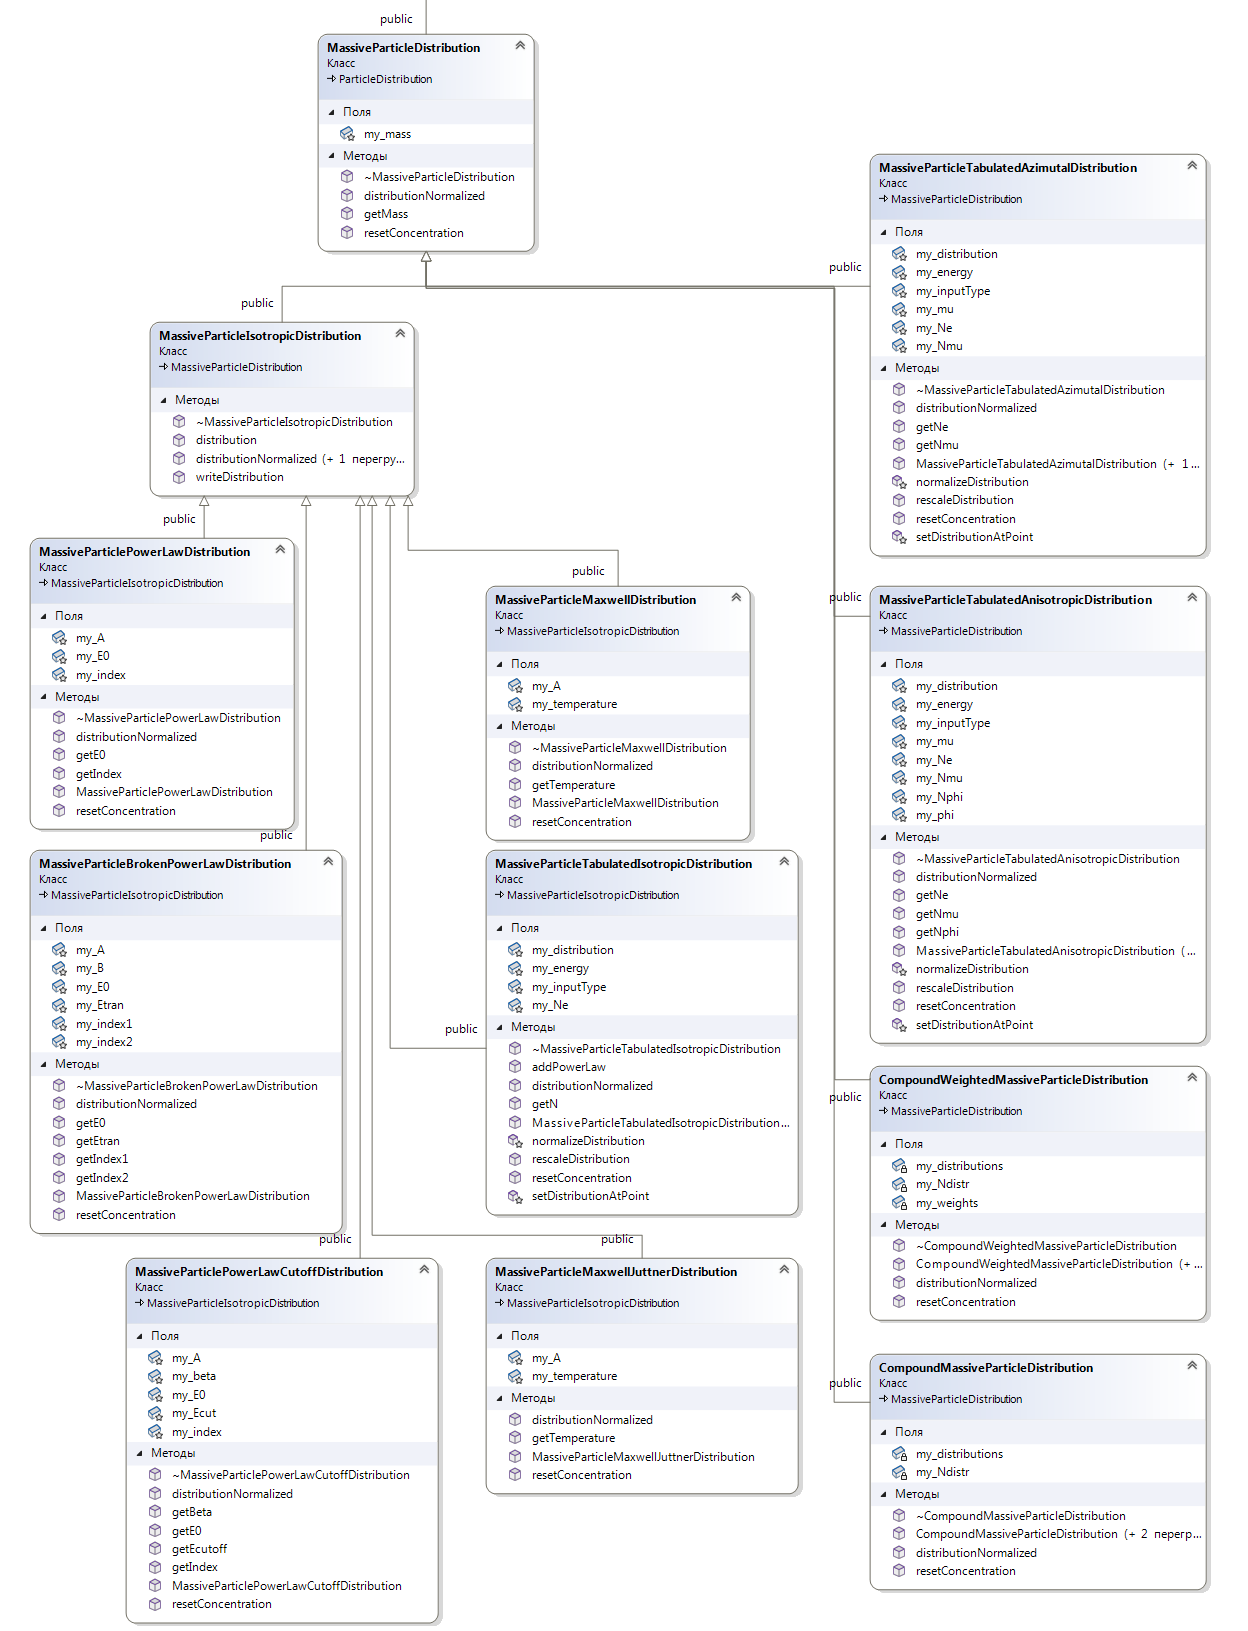
\includegraphics[width=14.5 cm]{./fig/massiveParticleDistribution1.png} 
	\caption{Схема наследования классов распределения массивных частиц}
	\label{massiveDistribution}
\end{figure}

Абстрактный класс изотропных распределений имеет шесть наследников, предназначенных для создания конкретных распределений: MassiveParticlePowerLawDistribution - для степенных распределений, MassiveParticleBrokenPowerLawDistribution - для степенных распределений с изломом, MassiveParticlePowerLawCutoffDistribution - для степенных распределений с экспоненциальным завалом, MassiveParticleMaxwellDistribution - для максвелловского распределения (обратите внимание, что в отличие от остальных распределений, максвелловское подразумевает под энергией только кинетическую энергию), MassiveParticleMaxwellJuttnerDistribution - для релятивистского распределения Максвелла-Юттнера и MassiveParticleTabulatedIsotropicDistribution - для таблично заданных распределений. 

Так же имеется четыре реализации анизотропных распределений: MassiveParticleTabulatedPolarDistribution - для таблично заданных распределений с зависимостью только от энергии и полярного угла, MassiveParticleAnisotropicDistribution - для таблично заданных распределений с зависимостью от всех переменных, CompoundMassiveParticleDistribution - для суммы распредлений общего вида, CompoundWeightedMassiveParticleDistribution - для взвешенной суммы распределений общего вида. В некоторых случаях оперировать весами распределений удобнее, чем непосредственно концентрациями. Полная схема наследования классов распределений массивных частиц представлена на рисунке \ref{massiveDistribution}, список публичных методов классов распределений массивных частиц приведен в Таблице \ref{MassiveParticleMethods1}. Пользователь может сам реализовывать необходимые ему виды распределений излучающих частиц, создав наследника класса MassiveParticleDistribution или MassiveParticleIsotropicDistribution и определив необходимые виртуальные методы.

\subsection{Считывание распределений из файла}
Классы таблично-заданных распределений, такие как например MassiveParticleTabulatedIsotropicDistribution, имеют конструктор принимающие на вход имена файлов, из которых будет считана функция распределения. Это должны быть текстовые файлы, содержащие таблицы с данными, причем формат единиц, в которых измеряется функция распределения может быть разным. Для задания формата входных файлов используется перечислимы тип DistributionInputType, имеющий пять значений:

\begin{itemize}
	\item ENERGY\_FE - во входных файлах заданы энергия и функция распределения по энергии
	\item ENERGY\_KIN\_FE - заданы кинетическая энергия и функция распределения по энергии
	\item GAMMA\_FGAMMA - задан лоренц-фактор и функция распределения по нему
	\item GAMMA\_KIN\_FGAMMA - задан лоренц-фактор, уменьшенный на единицу, и функция распределения по нему
	\item MOMENTUM\_FP - задан импульс и функция распределения по импульсу
\end{itemize}

Вне зависимости от формата входного файла, функция распределения будет преобразована к единицам энергия - распределение по энергии. С помощью этих параметров можно считывать табличные распределения из файлов, например так:

\begin{lstlisting}[language=c++]
	double electronConcentration = 1.0;
	int N = 100;
	MassiveParticleIsotropicDistribution* distribution = new
	MassiveParticleTabulatedIsotropicDistribution(massElectron,
	"energy.dat", "distribution.dat", N, electronConcentration,
	DistributionInputType::ENERGY_FE);
\end{lstlisting}

Для облегчения создания распределений из файла в сложных случаях реализован класс MassiveParticleDistributionFactory. У него есть несколько методов, позволяющих считывать целые серии распределений из набора пронумерованных файлов. Что может быть полезно, если функция распределения зависит от некоторого параметра, как в примере вычисления синхротронного излучения описанном в следующей главе \ref{}. Считать серию из десяти распределений электронов, содержащихся в файлах с именами  "Fe0.dat"\ , "Fe1.dat"\  и так далее, состоящих из двух колонок - лоренц-фактор и функция распределения, и добавить к этим распределениям степенной хвост с показателем 3, начиная с энергий в 100 энергий покоя можно вызовом одной функции: 

\begin{lstlisting}[language=c++]
	double electronConcentration = 1.0;
	int Nenergy = 100;
	int Ndistribution = 100;
	double powerLawEnergy = 100*me_c2;
	double index = 3.0;
	MassiveParticleIsotropicDistribution** distributions = 
	MassiveParticleDistributionFactory::
	readTabulatedIsotropicDistributionsAddPowerLawTail(
	massElectron, "./input/Fe", ".dat", Ndistribution, 
	DistributionInputType::GAMMA_FGAMMA, electronConcentration, Nenergy,
	powerLawEnergy, index);
\end{lstlisting}

Так же у пользователя есть возможность использовать конструкторы табличных распределений, принимающие не имена файлов, а непосредственно массивы со значениями функции распределения, которые пользователь создать любым удобным ему способом.

\begin{small}
	\topcaption{Публичные методы классов распределений массивных частиц }
	\label{MassiveParticleMethods1}
	\begin{xtabular}{|p{0.52\textwidth}|p{0.48\textwidth}|}
		\hline
		\textbf{MassiveParticlePowerLawDistribution} & Класс для степенного распределения\\
		\hline
		MassiveParticlePowerLawDistribution( const double\& mass, const double\& index, const double\& E0, const double\& concentration) & конструктор, создает экземпляр степенного распределния частиц с заданными массой, степенным индексом, начальной энергией распределения и полной концентрацией\\
		\hline
		getIndex() & возвращает степенной индекс распределения\\
		\hline
		getE0() & возвращает начальную энергию распределения\\
		\hline
		\textbf{MassiveParticleBrokenPowerLawDistribution} & Класс для степенного распределения с изломом\\
		\hline
		MassiveParticleBrokenPowerLawDistribution( const double\& mass, const double\& index1, const double\& index2, const double\& E0, const double\& Etran, const double\& concentration) & конструктор, создает экземпляр степенного распределния с изломом частиц с заданными массой, степенными индексоми на низких и высоких энергиях, начальной энергией распределения, энергией соответствующей излому и полной концентрацией\\
		\hline
		getIndex1() & возвращает степенной индекс распределения на низких энергиях\\
		\hline
		getIndex2() & возвращает степенной индекс распределения на высоких энергиях\\
		\hline
		getE0() & возвращает начальную энергию распределения\\
		\hline
		getEtran() & возвращает энергию излома\\
		\hline
		\textbf{MassiveParticlePowerLawCutoffDistribution} & Класс для степенного распределения с экспоненциальным завалом\\
		\hline
		MassiveParticlePowerLawCutoffDistribution(const double\& mass, const double\& index, const double\& E0, const double\& beta, const double\& Ecut, const double\& concentration) & конструктор, создает экземпляр степенного распределния с экспоненциальным завалом частиц с заданными массой, степенным индексом, начальной энергией распределения, параметром завала, энергией завала и полной концентрацией. $F(E)\propto (E/E_0)^{-index}\cdot\exp(-(E/E_{cut})^\beta)$\\
		\hline
		getIndex() & возвращает степенной индекс распределения \\
		\hline
		getBeta() & возвращает параметр завала распределения \\
		\hline
		getE0() & возвращает начальную энергию распределения\\
		\hline
		getEcutoff() & возвращает энергию экспоненциального завала\\
		\hline
		\textbf{MassiveParticleMaxwellDistribution} & Класс для распределения Максвелла\\
		\hline
		MassiveParticleMaxwellDistribution( const double\& mass, const double\& temperature, const double\& concentration) & конструктор, создает экземпляр распределния Максвелла частиц с заданными массой, температурой и полной концентрацией\\
		\hline
		getTemperature() & возвращает температуру распределения\\
		\hline
		\textbf{MassiveParticleMaxwellJuttnerDistribution} & Класс для распределения Максвелла-Юттнера\\
		\hline
		MassiveParticleMaxwellJuttnerDistribution( const double\& mass, const double\& temperature, const double\& concentration) & конструктор, создает экземпляр распределния Максвелла-Юттнера частиц с заданными массой, температурой и полной концентрацией\\
		\hline
		getTemperature() & возвращает температуру распределения\\
		\hline
		\textbf{MassiveParticleTabulatedIsotropicDistribution} & Класс для таблично заданного изотропного распределения\\
		\hline
		MassiveParticleTabulatedIsotropicDistribution( const double\& mass, const char* fileName, const int N, const double\& concentration, DistributionInputType inputType) & конструктор, создает экземпляр табличного распределния частиц с заданными массой и полной концентрацией с помощью указанного файла, состоящего из двух колнок с данными указанной длины. Так же указывается формат входных данных.\\
		\hline
		MassiveParticleTabulatedIsotropicDistribution( const double\& mass, const char* energyFileName, const char* distributionFileName, const int N, const double\& concentration, DistributionInputType inputType) & конструктор, создает экземпляр табличного распределния частиц с заданными массой и полной концентрацией с помощью указанных двух файлов, состоящих из колнок с данными указанной длины. Так же указывается формат входных данных. \\
		\hline
		MassiveParticleTabulatedIsotropicDistribution( const double\& mass, const double* energy, const double* distribution, const int N, const double\& concentration, DistributionInputType inputType) & конструктор, создает экземпляр табличного распределния частиц с заданными массой и полной концентрацией с помощью двух переданных массивов данных указанной длины. Так же указывается формат входных данных.\\
		\hline
		getN() & возвращает количество ячеек в таблице задающей функцию\\
		\hline
		getEmin() & возвращает минимальную энергию распределения\\
		\hline
		getEmax() & возвращает максимальную энергию распределения\\
		\hline
		rescaleDistribution(const double\& k) & масштабирует распределение, вытягивая его по оси энергии по формуле $E' = mc^2 + k\cdot(E-mc^2)$, $F(E')=F(E)/k$. Данная функция может быть полезна, например, в случае когда исходная функция распределения получена в результате работы численного кода с измененной массой электронов\\
		\hline
		addPowerLaw( const double\& Epower, const double\& index) & добавляет к функции распределения степенной с указанным индексом, начиная с указанной энергии. Функция распределения при этом остается нормированной на указанную ранее концентрацию\\
		\hline 
		\textbf{MassiveParticleTabulatedPolarDistribution} & Класс для таблично заданного распределения с зависимостью от полярного угла\\
		\hline
		MassiveParticleTabulatedPolarDistribution( const double\& mass, const char* energyFileName, const char* muFileName, const char* distributionFileName, const int Ne, const int Nmu, const double\& concentration, DistributionInputType inputType) & конструктор, создает экземпляр табличного распределния частиц с заданными массой и полной концентрацией с помощью  трех указанных файлов, в двух из которых содержатся сетки по энергии и косинусу полярного угла с указанными размерами, а в третьем двумерный массив функции распределения. Так же указывается формат входных данных.\\
		\hline
		MassiveParticleTabulatedPolarDistribution( const double\& mass, const double* energy, const double* mu, const double** distribution, const int Ne, const int Nmu, const double\& concentration, DistributionInputType inputType) & конструктор, создает экземпляр табличного распределния частиц с заданными массой и полной концентрацией с помощью трех переданных массивов данных, в двух из которых содержатся сетки по энергии и косинусу полярного угла с указанными размерами, а в третьем двумерный массив функции распределения. Так же указывается формат входных данных.\\
		\hline
		getNe() & возвращает количество ячеек по энергии в таблице задающей функцию распределения\\
		\hline
		getEmin() & возвращает минимальную энергию распределения\\
		\hline
		getEmax() & возвращает максимальную энергию распределения\\
		\hline
		getNmu() & возвращает количество ячеек по полярному углу в таблице задающей функцию распределения\\
		\hline
		rescaleDistribution(const double\& k) & масштабирует распределение, вытягивая его по оси энергии по формуле $E' = mc^2 + k\cdot(E-mc^2)$, $F(E',\mu)=F(E,\mu)/k$. Данная функция может быть полезна, например, в случае когда исходная функция распределения получена в результате работы численного кода с измененной массой электронов\\
		\hline
		\textbf{MassiveParticleTabulatedAnisotropicDistribution} & Класс для таблично заданного анизотропного распределения общего вида\\
		\hline
		MassiveParticleTabulatedAnisotropicDistribution( const double\& mass, const char* energyFileName, const char* muFileName, const char* distributionFileName, const int Ne, const int Nmu, const int Nphi, const double\& concentration, DistributionInputType inputType) & конструктор, создает экземпляр табличного распределния частиц с заданными массой и полной концентрацией с помощью  трех указанных файлов, в двух из которых содержатся сетки по энергии и косинусу полярного угла с указанными размерами, а в третьем двумерный массив функции распределения. Сетка по азимутальному углу считается расномерной и определяется только размером. Так же указывается формат входных данных.\\
		\hline
		MassiveParticleTabulatedAnisotropicDistribution( const double\& mass, const double* energy, const double* mu, const double*** distribution, const int Ne, const int Nmu, const int Nphi, const double\& concentration, DistributionInputType inputType) & конструктор, создает экземпляр табличного распределния частиц с заданными массой и полной концентрацией с помощью трех переданных массивов данных, в двух из которых содержатся сетки по энергии и косинусу полярного угла с указанными размерами, а в третьем двумерный массив функции распределения. Сетка по азимутальному углу считается расномерной и определяется только размером. Так же указывается формат входных данных.\\
		\hline
		getNe() & возвращает количество ячеек по энергии в таблице задающей функцию распределения\\
		\hline
		getEmin() & возвращает минимальную энергию распределения\\
		\hline
		getEmax() & возвращает максимальную энергию распределения\\
		\hline
		getNmu() & возвращает количество ячеек по полярному углу в таблице задающей функцию распределения\\
		\hline
		getNphi() & возвращает количество ячеек по азимутальному углу в таблице задающей функцию распределения\\
		\hline
		rescaleDistribution(const double\& k) & масштабирует распределение, вытягивая его по оси энергии по формуле $E' = mc^2 + k\cdot(E-mc^2)$, $F(E',\mu, \phi)=F(E,\mu, \phi)/k$. Данная функция может быть полезна, например, в случае когда исходная функция распределения получена в результате работы численного кода с измененной массой электронов\\
		\hline
		\textbf{CompoundMassiveParticleDistribution} & Класс для распределения, состоящего из суммы других распределений\\
		\hline
		CompoundMassiveParticleDistribution( int N, MassiveParticleDistribution** distributions) & конструктор, создает экземпляр класса содержащий смесь заданного количества указанных распределений\\
		\hline
		CompoundMassiveParticleDistribution( MassiveParticleDistribution* dist1, MassiveParticleDistribution* dist2) & конструктор, создает экземпляр класса, содержащий смесь двух распределений \\
		\hline
		CompoundMassiveParticleDistribution( MassiveParticleDistribution* dist1, MassiveParticleDistribution* dist2, MassiveParticleDistribution* dist3) & конструктор, создает экземпляр класса, содержащий смесь трех распределений\\
		\hline
		\textbf{CompoundWeightedMassiveParticleDistribution} & Класс для распределения, состоящего из взвешенной суммы других распределений \\
		\hline
		CompoundWeightedMassiveParticleDistribution( int N, const double* weights, MassiveParticleDistribution** distributions) & конструктор, создает экземпляр класса содержащий смесь заданного количества указанных распределений с заданными весами \\
		\hline
		CompoundWeightedMassiveParticleDistribution( MassiveParticleDistribution* dist1, const double\& w1, MassiveParticleDistribution* dist2, const double\& w2) & конструктор, создает экземпляр класса, содержащий смесь двух распределений с указанными весами \\
		\hline
		CompoundWeightedMassiveParticleDistribution( MassiveParticleDistribution* dist1, const double\& w1, MassiveParticleDistribution* dist2, const double\& w2, MassiveParticleDistribution* dist3, const double\& w3) & конструктор, создает экземпляр класса, содержащий смесь трех распределений с указанными весами \\
		\hline
				
	\end{xtabular}
\end{small}

\section{Источники излучения}

В коде FAINA есть возможность расчета излучения, используя на прямую функции распределения излучающих частиц, с указанием необходимых дополнительных параметров, таких как объем источника, расстояние до него, магнитное поле и других. Но более универсальным и рекомендованным способ является расчет с помощью создания модели источника излучения. При таком подходе возможно учесть геометрическое строение источника, его неоднородности и другие особенности.

Реализованы два базовых класса источников - независящие от времени, представленные абстрактным классом RadiationSource, и изменяющиеся со временем, представленные абстрактным классом RadiationTimeDependentSource. Эти два класса не связаны между собой через наследование, но объект первого класса содержится внутри объектов второго как приватное поле класса. Схема классов источников излучения представлена на рисунке \ref{radiationSource}.

\begin{figure}
	\centering
	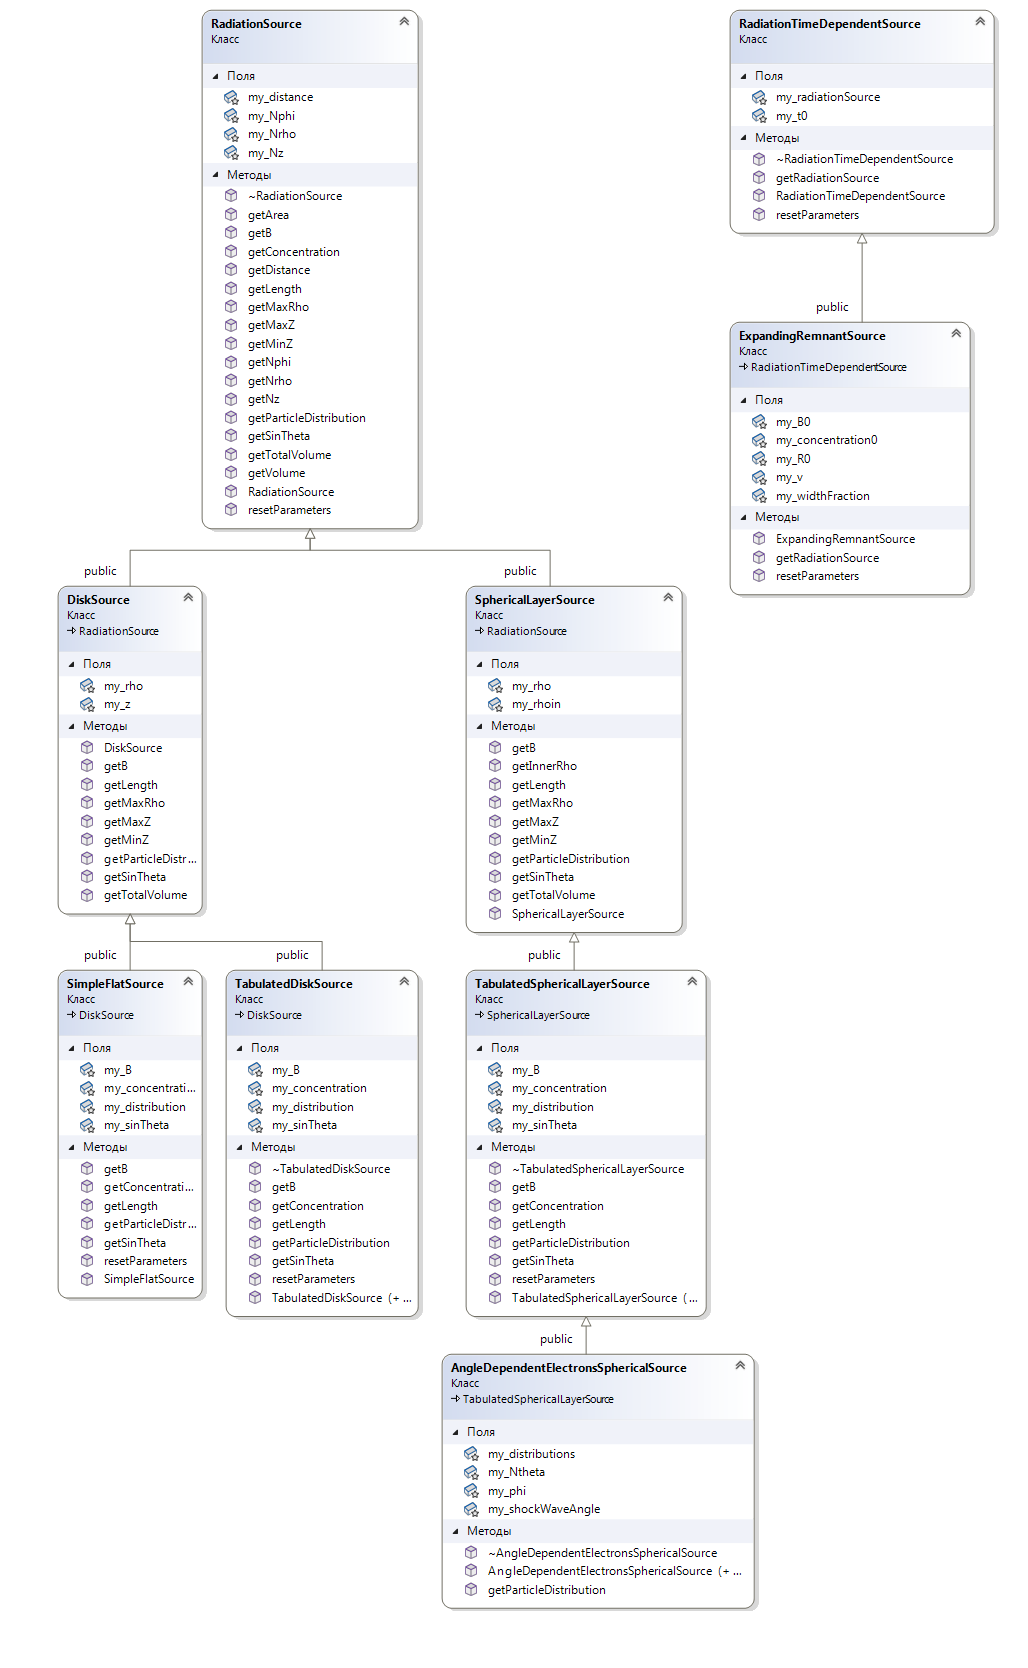
\includegraphics[width=14.5 cm]{./fig/radiationSource.png} 
	\caption{Схема наследования классов источников излучения}
	\label{radiationSource}
\end{figure}

\subsection{Источники излучения, не зависящие от времени}
Источники излучения без временной зависимости реализованы с помощью абстрактного класса RadiationSource. Геометрически каждый источник задан в виде пространственной области в цилиндрических координатах, с осью z направленной вдоль луча зрения к наблюдателю, и характеризуется максимальным радиусом и минимальным и максимальным значением координаты z. Такая система координат выбрана для удобства учета процессов поглощения при прохождении излучения внутри самого источника вдоль луча зрения. Отличие реальной формы источника от цилиндрической реализовано с помощью долей заполнения веществом источника ячеек пространственной сетки. Модель источника, имеющего форму шарового слоя, в цилиндрическо пространственной сетке изображена на рисунке \ref{sphericalLayer}. Цветом обозначена доля объема ячейки, заполненная веществом источника.

\begin{figure}
	\centering
	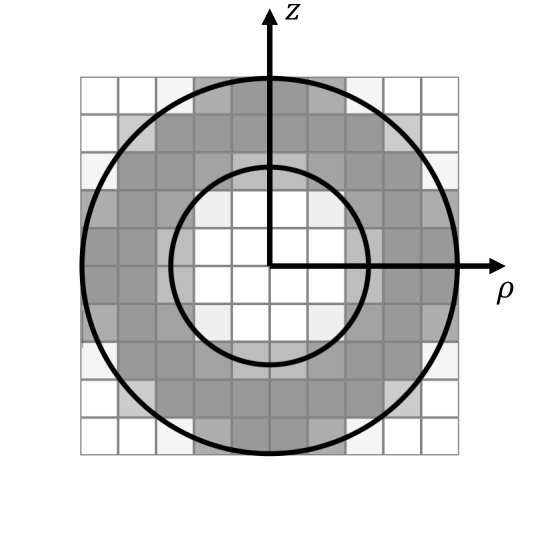
\includegraphics[width=10.5 cm]{./fig/sphericalSource.png} 
	\caption{Модель источника в форме шарового слоя, помещенного в цилиндрическую пространственную координатную сетку. Цвет характеризует долю объема ячейки, заполненную веществом источника.}
	\label{sphericalLayer}
\end{figure}

Так же источники излучения имеют следующие важные характеристки, которые могут меняться в различных пространственных ячейках источника: концентрация излучающих частиц, их функция распределения, магнитное поле и угол его наклона к лучу зрения. Большинство методов расчета излучения (все кроме обратного комптоновского рассеяния) реализованы только для изотропных распределений излучающих частиц, поэтому источники содержат только изотропные распределения. Так же у источника должно быть задано расстояние до наблюдателя.

Класс RadiationSource имеет два абстрактных класса-наследника: DiskSource - для источников в форме диска, перпендикулярного лучу зрения, и SphericalLayerSource - для источников в форме шарового слоя. Источники в форме диска имеют две реализации: SimpleFlatSource - однородный диск, состоящий из одной пространственной ячейки с заданными параметрами, и TabulatedDiskSource - источник, в котором все характеристики таблично заданы на пространственной сетке. Источники в форме шарового слоя имеют следующие реализации: TabulatedSphericalSource - источник, в котором все характеристики таблично заданы на пространственной сетке, и отнаследованный от него AngleDependentElectronsSphericalSource. Последний класс нужен для реализации важного в астрофизике случая, когда функция распределения излучающих частиц зависит от угла наклона магнитного поля по отношению к направлению распространения ударной волны \cite{SironiSpitkovsky2009pair, GuoSironi2014_1,Crumley2019, Romansky2018, еще}. В данном источнике такие параметры, как концентрация, магнитное поле и его угол наклона к лучу зрения заданы таблично на пространственной сетке, а функция распределения излучающих частиц - в виде таблицы по углам наклона магнитного поля к направлению распространения ударной волны, которая в данном случае считается сферически симметричной. Функция распределения в каждой ячейке выбирается в зависимости от вычисленного угла наклона магнитного поля к ударной волне. Публичные методы классов источников излучения без зависимости от времени перечислены в Таблице \ref{sourceMethods1}.

\begin{small}
	\topcaption{Публичные методы классов источников излучения без зависимости от времени }
	\label{sourceMethods1}
	\begin{xtabular}{|p{0.5\textwidth}|p{0.5\textwidth}|}
		\hline
		\textbf{RadiationSource} & абстрактный класс для источников излучения общего вида\\
		\hline
		virtual getMaxRho() & чисто виртуальный метод, возвращает максимальный цилиндрический радиус источника\\
		\hline
		virtual getMinZ() & чисто виртуальный метод, возвращает минимальную границу источника по оси z\\
		\hline
		virtual getMaxZ() & чисто виртуальный метод, возвращает максимальную границу источника по оси z\\
		\hline
		getNrho() & возвращает количество пространственных ячеек по радиальной оси цилиндрических координат\\
		\hline
		getNz() & возвращает количество пространственных ячеек по оси z цилиндрических координат\\
		\hline
		getNphi() & возвращает количество пространственных ячеек по по азимутальному углу цилиндрических координат\\
		\hline
		getDistance() & возвращает расстояние до источника\\
		\hline
		getArea(int irho) & возвращает поперечное сечение данной пространственной ячейки\\
		\hline
		getVolume(int irho, int iz, int iphi) & возвращает объем ячейки, занятый веществом источника. Этот метод согласован с методами getArea и getLength и возвращает их произведение\\
		\hline
		virtual getB(int irho, int iz, int iphi) & чисто виртуальный метод, возвращает значение магнитного поля в ячейке\\
		\hline
		virtual getConcentration(int irho, int iz, int iphi) & чисто виртуальный метод, возвращает значение концентрации в ячейке \\
		\hline
		virtual getSinTheta(int irho, int iz, int iphi) & чисто виртуальный метод, возвращает синус угла наклона магнитного поля к лучу зрения\\
		\hline
		virtual getTotalVolume() & чисто виртуальный метод, возвращает полный объем источника\\
		\hline
		virtual getLength(int irho, int iz, int iphi) & чисто виртуальный метод, возвращает среднюю толщину ячейки, заполненную веществом источника\\
		\hline
		virtual resetParameters(const double* parameters, const double* normalizationUnits) & чисто виртуальный метод, меняющий параметры источника. Список параметров, их количество, их влияние на источник определяются пользователем в конкретных реализациях класса. Принимет массив параметров и массив единиц в которых они измеряны. Данный метод используется в процедурах оптимизации, либо при учете изменения источника со временем\\
		\hline
		virtual getParticleDistribution(int irho, int iz, int iphi) & чисто виртуальный метод, возвращает распределение излучающих частиц в ячейке\\
		\hline
		\textbf{DiskSource} & Абстрактный класс для источников в форме диска\\
		\hline
		\textbf{SimpleFlatSource} & Класс для источников в форме однородного диска\\
		\hline
		SimpleFlatSource( MassiveParticleIsotropicDistribution* electronDistribution, const double\& B, const double\& sinTheta, const double\& rho, const double\& z, const double\& distance) & конструктор, возвращает экземпляр с заданными распределением частиц, магнитным полем, синусом угла его наклона, радиусом диска, толщиной диска и расстоянием до источника\\
		\hline
		\textbf{TabulatedDiskSource} & Класс для источников в форме диска с таблично заданными значениями параметров\\
		\hline
		TabulatedDiskSource( int Nrho, int Nz, int Nphi, MassiveParticleIsotropicDistribution* electronDistribution, double*** B, double*** sinTheta, double*** concentration, const double\& rho, const double\& z, const double\& distance) & конструктор, возвращает экземпляр с заданными с помощью массивов распределением частиц, магнитным полем, синусом угла его наклона, а так же заданными радиусом диска, толщиной диска и расстоянием до источника\\
		\hline
		TabulatedDiskSource( int Nrho, int Nz, int Nphi, MassiveParticleIsotropicDistribution* electronDistribution, const double\& B, const double\& sinTheta, const double\& concentration , const double\& rho, const double\& z, const double\& distance) & конструктор, возвращает экземпляр с заданными однородными распределением частиц, магнитным полем, синусом угла его наклона, а так же заданными радиусом диска, толщиной диска и расстоянием до источника\\
		\hline
		\textbf{SphericalLayerSource} & Абстрактный класс для источников в форме шарового слоя\\
		\hline
		double getInnerRho() & возвращает внутренний радиус шарового слоя\\
		\hline
		\textbf{TabulatedSphericalLayerSource} & Класс для источников в форме шарового слоя с таблично заданными значениями параметров\\
		\hline
		TabulatedSphericalLayerSource(int Nrho, int Nz, int Nphi, MassiveParticleIsotropicDistribution* electronDistribution, double*** B, double*** sinTheta, double*** concentration, const double\& rho, const double\& rhoin, const double\& distance) & конструктор, возвращает экземпляр с заданными с помощью массивов распределением частиц, магнитным полем, синусом угла его наклона к лучу зрения, а так же заданными внешним и внутренним радиусом диска и расстоянием до источника\\
		\hline
		TabulatedSphericalLayerSource(int Nrho, int Nz, int Nphi, MassiveParticleIsotropicDistribution* electronDistribution, const double\& B, const double\& concentration, const double\& sinTheta, const double\& rho, const double\& rhoin, const double\& distance) &  конструктор, возвращает экземпляр с заданными однородными распределением частиц, магнитным полем, синусом угла его наклона, а так же заданными внутренним и внешним радиусом диска и расстоянием до источника \\
		\hline
		\textbf{AngleDependentElectronsSphericalSource} & Класс для источников в форме шарового слоя с таблично заданными значениями концентрации и магнитного поля и функцией распределения излучающих частиц, зависящей от угла наклона магнитного поля к направлению распространения ударной волны\\
		\hline
		AngleDependentElectronsSphericalSource( int Nrho, int Nz, int Nphi, int Ntheta, MassiveParticleIsotropicDistribution** electronDistributions, double*** B, double*** sinTheta, double*** phi, double*** concentration, const double\& rho, const double\& rhoin, const double\& distance) & конструктор, возвращает экземпляр с заданными с помощью массивов магнитным полем, синусом угла его наклона к лучу зрения, а так же заданными внешним и внутренним радиусом диска и расстоянием до источника. Распределение частиц задается в виде массива табличных значений в зависимости от угла наклона магнитного поля к направлению распространения ударной волны\\
		\hline
		AngleDependentElectronsSphericalSource(int Nrho, int Nz, int Nphi, int Ntheta, MassiveParticleIsotropicDistribution** electronDistributions, const double\& B, const double\& sinTheta, const double\& phi, const double\& concentration, const double\& rho, const double\& rhoin, const double\& distance) & конструктор, возвращает экземпляр с заданными однородными  магнитным полем, синусом угла его наклона, а так же заданными внутренним и внешним радиусом диска и расстоянием до источника. Распределение частиц задается в виде массива табличных значений в зависимости от угла наклона магнитного поля к направлению распространения ударной волны\\
		\hline
	\end{xtabular}
\end{small}

\subsection{Источники излучения, меняющиеся со временем}
Источники излучения, учитывающие зависимость от времени, представлены абастрактным классом классом RadiationTimeDependentSource. Этот класс не является наследником класса RadiationSource, но содержит экземпляр такого класса внутри себя, чтобы использовать его для расчета излучения в конкретный момент времени. В текущей версии кода реализован только один наследник RadiationTimeDependentSource - ExpandingRemnantSource, представляющий собой модель расширяющегося остатка сверхновой. В данной модели предполагается, что размер источника увеличивается во времени с постоянной скоростью, магнитное поле падает обратно пропорционально размеру источника, концентрация обратно пропорционально квадрату размера а толщина шарового слоя остается постоянной. Пользователь может создавать свои классы источников с другими зависимостями параметров от времени. Публичные методы классов RadiationTimeDependentSource и ExpandingRemnantSource перечислены  в Таблице \ref{sourceTimeDependentMethods1}.

\begin{small}
	\topcaption{Публичные методы классов источников излучения учитывающих зависимость от времени }
	\label{sourceTimeDependentMethods1}
	\begin{xtabular}{|p{0.5\textwidth}|p{0.5\textwidth}|}
		\hline
		\textbf{RadiationTimeDependentSource} & Абстрактный класс для учета изменений источников излучения со временем\\
		\hline
		virtual resetParameters(const double* parameters, const double* normalizationUnits) & чисто виртуальный метод, меняющий параметры источника. Список параметров, их количество, их влияние на источник определяются пользователем в конкретных реализациях класса. Принимет массив параметров и массив единиц в которых они измеряны. Данный метод применяется в процедурах оптимизации\\
		\hline
		virtual getRadiationSource(double\& time, const double* normalizationUnits) & возвращает источник излучения с параметрами соответствующими заданному моменту времени. Так же принимает на вход массив единиц, в которых измеряются параметры этого источника.\\
		\hline
		\textbf{ExpandingRemnantSource} & класс, представляющий модель расширяющегося с постоянной скоростью остатка сверхновой, имеющего форму шарового слоя постоянной толщины с однородными концентрацией и магнитным полем \\
		\hline
		ExpandingRemnantSource(const double\& R0, const double\& B0, const double\& concentration0, const double\& v, const double\& widthFraction, RadiationSource* source, const double\& t0) & конструктор, создает экземпляр класса расширяющейся сферической оболочки с заданными в момент t0 радиусом, магнитным полем, концентрацией, скоростью расширения, отношением толщины оболочки к радиусу и моделью источника. Для коректного учета изменения источника во времени важно, чтобы конретная реализация метода source->resetParameters соответствовала той,что используется в методе getRadiationSource. В данном случае подходят все перечисленные выше реализации источников не зависящих от времени\\
		\hline
	\end{xtabular}
\end{small}

\section{Вычисление излучения}

Для расчета излучения источников используется класс RadiationEvaluator и его наследники. Список публичных методов этого класса приведен в Таблице \ref{radiationEvaluator}. Общая схема расчета излучения такова: создать источник излучения, используя один из классов описанных в предыдущем разделе или написанный самостоятельно, затем создать вычислитель излучения нужного типа, и вызвать у него метод evaluateFluxFromSource(const double\& photonFinalEnergy, RadiationSource* source), вычисляющую энергетическую плотность потока излучения источника на данной энергии принимаемого фотона в единицах  $\text{см}^{-2} \text{с}^{-1}$. Далее в данном разделе описаны реализации класса RadiationEvaluator для конкретных видов излучения. Схема наследования классов вычислителей излучения представлена на рисунке \ref{radiationEvaluators}. Физическая сторона вопроса, формулы по которым расчитывается излучение подробно описаны в Главе \ref{Formulae}.

\begin{table}
	\begin{center}
		\begin{small}
	\caption{Публичные методы классa RadiationEvaluator }
	\label{radiationEvaluator}
	\begin{xtabular}{|p{0.5\textwidth}|p{0.5\textwidth}|} 
		\hline
		\textbf{RadiationEvaluator} & абстрактный класс для вычисления излучения \\
		\hline
		virtual evaluateFluxFromIsotropicFunction( const double\& photonFinalEnergy, MassiveParticleIsotropicDistribution* electronDistribution, const double\& volume, const double\& distance) & чисто виртуальный метод, возвращает энергетическую плотность потока излучаемого элементарным объемом с источника с данным распределением, на данном расстоянии от наблюдателя в единицах $\text{см}^{-2} \text{с}^{-1}$. Данный метод лучше не использовать самостоятельно, использовать вместо него расчет излучения от источников\\
		\hline
		virtual evaluateFluxFromSource(const double\& photonFinalEnergy, RadiationSource* source) & чисто виртуальный метод, возвращает энергетическую плотность потока излучаемого данным источником в единицах $\text{см}^{-2} \text{с}^{-1}$ \\
		\hline
		virtual resetParameters( const double* parameters, const double* normalizationUnits) & чисто виртуальный метод, позволяет изменить внутренние параметры вычислителя излучения. Список параметров, их количество, их влияние на источник определяются  в конкретных реализациях класса, данный метод используется при оптимизации\\
		\hline
		writeFluxFromSourceToFile(const char* fileName, RadiationSource* source, const double\& Ephmin, const double\& Ephmax, const int Nph) & записывает в файл с данным именем излучение источника в единицах $\text{см}^{-2} \text{с}^{-1}$ в диапазоне от минимальной до максимальной энергии, с заданным количеством точек, распределенных логарифмически\\
		\hline
	\end{xtabular}
\end{small}
\end{center}
\end{table}

\begin{figure}
	\centering
	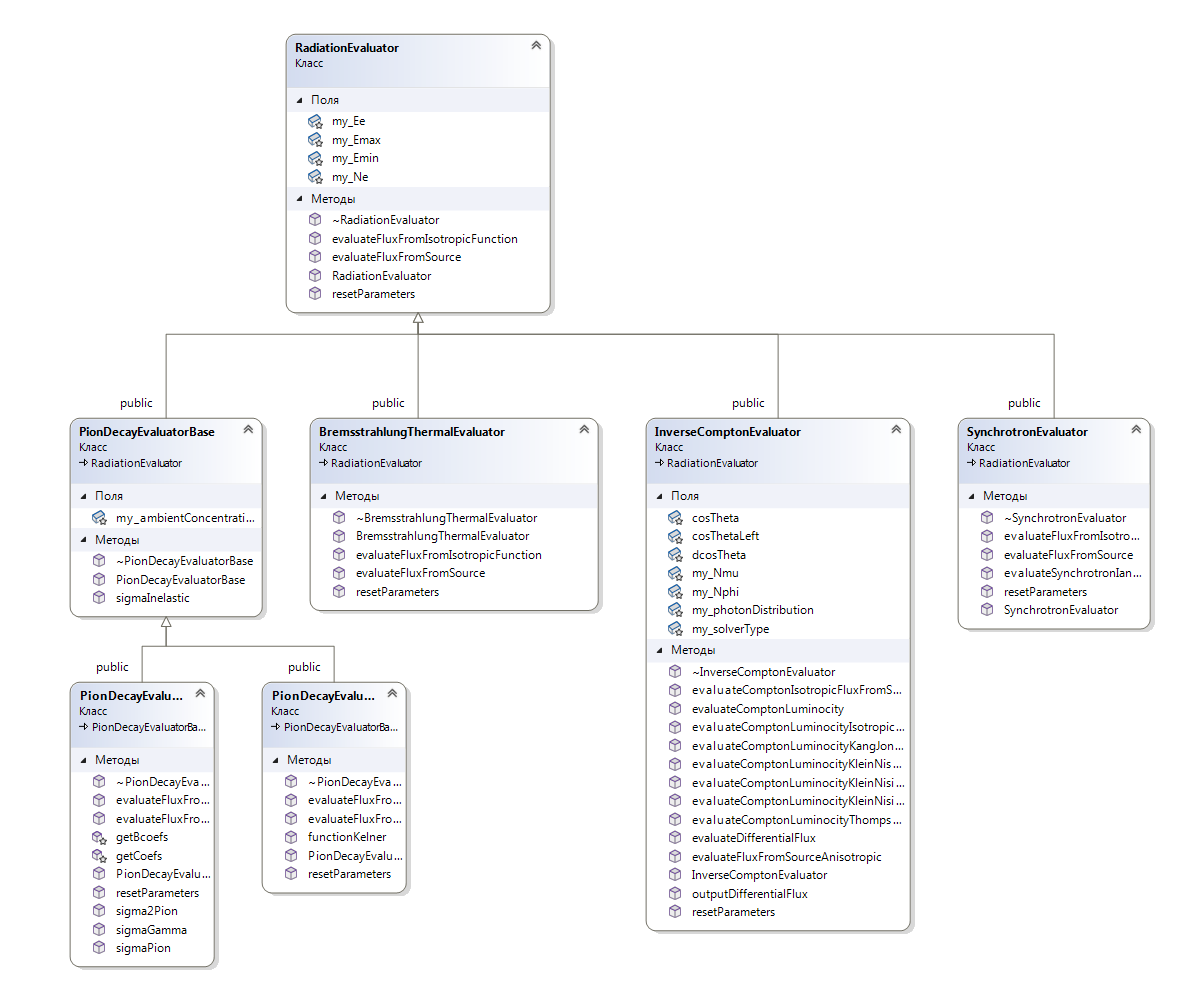
\includegraphics[width=10.5 cm]{./fig/radiationEvaluator.png} 
	\caption{Схема наследования классов вычислителей излучения.}
	\label{radiationEvaluators}
\end{figure}

\subsection{Синхротронное излучение}
Для расчета синхротронного излучения используется класс SynchrotronEvaluator. В нем используется приближение непрерывного спектра, то есть рассматриваемые частоты фотонов предполагаются намного большими, чем частота вращения излучающих частиц в магнитном поле. Реализован случай только изотропной функции распределения излучающих частиц. Так же возможен учет синхротронного самопоглощения. Используемая геометрия источников, показанная на рисунке \ref{sphericalLayer}, позволяет легко интегрировать излучение по лучу зрения, и учитывать при этом поглощение внутри источника. При создании объекта класса необходимо указать рассматриваемый диапазон энергий частиц и количество точек в нем, параметр отвечающиза учет самопоглощения (значение по умолчанию true), а так же значения магнитного поля, синуса угла наклона к лучу зрения и толщины излучаемой области, которые будут использоваться в случае расчета излучения без указания источника, а только с использованием распределения частиц. Публичные методы класса SynchrotronEvaluator перечислены в Таблице \ref{SynchrotronEvaluator}. Пример вычисления синхотронного излучения приведен в разделе \ref{quickStart}.
\begin{table}
	\begin{center}
	\begin{small}
	\caption{Публичные методы классa SynchrotronEvaluator }
	\label{SynchrotronEvaluator}
	\begin{tabularx}{\textwidth}{|X|X|} 
		\hline
		\textbf{SynchrotronEvaluator} & класс предназначенный для вычисления синхротронного излучения\\
		\hline
		SynchrotronEvaluator( int Ne, double Emin, double Emax, bool selfAbsorption = true, const double\& defaultB = 0, const double\& defaultSinTheta = 1.0, const double\& defaultLength = 0) & конструктор, создает экземпляр с указанным диапазоном рассматриваемых энергий, параметром учета самопоглощения, и значениями по умолчанию магнитного поля, его наклона и толщины\\
		\hline
		evaluateSynchrotronIandA(const double\& photonFinalFrequency, const double\& photonFinalTheta, const double\& photonFinalPhi, const double\& B, const double\& sinhi, const double\& concentration, MassiveParticleIsotropicDistribution* electronDistribution, double\& I, double\& A) & вычисляет значения излучательной способности и коэффициента поглощения распределения с данной концентрацией в данном магнитном поле\\
		\hline
	\end{tabularx}
\end{small}
\end{center}
\end{table}
\subsection{Обратное комптоновское рассеяние}
Для расчета излучения, получающегося в результате процесса обратного комптоновского рассеяния, использеутся класс InverseComptonEvaluator. Внутри него реализованы четыре различных метода расчета излучения, для обозначения которых используется перечислимый тип ComptonSolverType, имеющий следующие значения:

\begin{itemize}
	\item ISOTROPIC\_THOMSON - модель рассеяния в томсоновсков режиме. Реализовано только для степенного распределения электронов и теплового фотонов \cite{Ginzburg1975} глава 17, с 466
	\item ANISOTROPIC\_KLEIN\_NISHINA - модель расчитывающее излучение напрямую из сечения Клейна-Нишины, возможен учет анизотропных функций распределения \cite{KleinNishina, Dubus}
	\item ISOTROPIC\_KLEIN\_NISHINA - модель расчитывающее излучение напрямую из сечения Клейна-Нишины, но для изотропных функций распределения, что позволяет уменьшить количество интегрирований
	\item ISOTROPIC\_JONES - модель, использующая аналитически проинтегрированное по углам сечение Клейна-Нишины \cite{JonesCompton, BykovUvarov2000}
\end{itemize}

При создании объекта класса InverseComptomEvaluator необходимо указать рассматриваемый диапазон энергий частиц и количество точек в нем, количество ячеек в сетке по полярному и азимутальному углу, изотропную функцию распределения фотонов, которая будет использоваться по умолчанию и метод расчета излучения. Публичные методы класса SynchrotronEvaluator перечислены в Таблице \ref{InverseComptonEvaluator}.
\begin{table}[h]
	\begin{center}
		\begin{small}
	\caption{Публичные методы классa InverseComptonEvaluator }
	\label{InverseComptonEvaluator}
	\begin{tabularx}{\textwidth}{|X|X|} 
		\hline
		\textbf{InverseComptonEvaluator} & класс предназначенный для вычисления излучения рождащегося в результате обратного комптоновского рассеяния\\
		\hline
		InverseComptonEvaluator( int Ne, int Nmu, int Nphi, double Emin, double Emax, PhotonIsotropicDistribution* photonDistribution, ComptonSolverType solverType) & конструктор, создает экземпляр с заданным рассматриваемым диапазоном энергии, количеством ячеек в сетке по полярному и азимутальному углу, изотропной функцией распределения фотонов, которая будет использоваться по умолчанию и методом расчета излучения\\
		\hline
		evaluateComptonFluxKleinNishinaAnisotropic const double\& photonFinalEnergy, const double\& photonFinalTheta, const double\& photonFinalPhi, PhotonDistribution* photonDistribution, MassiveParticleDistribution* electronDistribution, const double\& volume, const double\& distance) & возвращает энергетическую плотность потока энергии в заданном направлении, излучением созданным заданными функциями распределения фотонов и рассеивющих частиц (которые могут быть анизотропными) в заданном объеме на данном расстоянии\\
		\hline
		evaluateFluxFromSourceAnisotropic( const double\& photonFinalEnergy, const double\& photonFinalTheta, const double\& photonFinalPhi, PhotonDistribution* photonDistribution, RadiationSource* source) & возвращает энергетическую плотность потока энергии в заданном направлении, излучением созданным заданными распределения фотонов и источником, содержащим распределения рассеивающих частиц\\
		\hline
	\end{tabularx}
\end{small}
\end{center}
\end{table}

Пример вычисления излучения от обратного комптоновского рассеяние содержится в процедуре evaluateComtonWithPowerLawDistribution() в файле main.cpp. В ней расчитывается рентгеновское излучение, исходящее от объекта CSS161010 при рассеивании степенного распределения электронов, определенного в работе \cite{Coppejans2020}, на среднегалактическом распределении фотонов.  Сначала определим переменные, задающие основные параметры источника - концентрацию частиц, его размер и магнитное поле. Для вычисления обратного комптоновского рассеяния магнитное поле не используется, но в источнике нужно его задать, поэтому положим его равным нулю. Так же зададим параметры сетки по энергиям и углам, которая будет использоваться вычислителем

\begin{lstlisting}[language=c++]
	double electronConcentration = 150;
	double sinTheta = 1.0;
	double rmax = 1.3E17;
	double B = 0.0;
	double distance = 150*1E6*parsec;
	
	double Emin = me_c2;
	double Emax = 1000 * me_c2;
	int Ne = 200;
	int Nmu = 20;
	int Nphi = 4;
\end{lstlisting}

Далее создадим распределение фотонов, воспользовавшись статическим методом класса MultiPlankDistribution getGalacticField, который возвращает среднегалактическое фотонное распределение, и распределение электронов - возьмем степенное рспределение с показателем 3.5.
\begin{lstlisting}[language=c++]
	PhotonIsotropicDistribution* photonDistribution = 
	    PhotonMultiPlankDistribution::getGalacticField();
	MassiveParticlePowerLawDistribution* electrons = new 
	    MassiveParticlePowerLawDistribution(massElectron, 3.5,
	    Emin, electronConcentration);
\end{lstlisting}

С помощью введенных ранее переменных создадим источник излучения и вычислитель излучения. В качестве метода расчета выберем самый универсальный - ANISOTROPIC\_KLEIN\_NISHINA

\begin{lstlisting}[language=c++]
	RadiationSource* source = new SimpleFlatSource(
	  electrons, B, sinTheta, rmax, rmax, distance);
	
	InverseComptonEvaluator* comptonEvaluator = new 
	    InverseComptonEvaluator(Ne, Nmu, Nphi, Emin, Emax, 
	    photonDistribution, ComptonSolverType::ANISOTROPIC_KLEIN_NISHINA);
\end{lstlisting}

Предположим, что мы не хотим пользоваться встроенным методом вывода излучения в файл, так как хотим получить конечный результат в других единицах, например энергию фотона измерят в электронвольтах, а поток вывести в формате $E F(E)$ - $\text{эрг}\text{см}^{-2}\text{с}^{-1}$. Создадим тогда сетку значений энергии фотонов
\begin{lstlisting}[language=c++]
	int Nnu = 200;
	double* E = new double[Nnu];
	double* F = new double[Nnu];
	double Ephmin = 0.01 * kBoltzman * 2.725;
	double Ephmax = 2 * Emax;
	double factor = pow(Ephmax / Ephmin, 1.0 / (Nnu - 1));
	E[0] = Ephmin;
	F[0] = 0;
	for (int i = 1; i < Nnu; ++i) {
		E[i] = E[i - 1] * factor;
		F[i] = 0;
	}
\end{lstlisting}
после этого вычислим в цикле желаемые потоки излучения
\begin{lstlisting}[language=c++]
	for (int i = 0; i < Nnu; ++i) {
		F[i] = comptonEvaluator->evaluateFluxFromSource(
		    E[i], source);
	}
\end{lstlisting}
и запишем их в файл, переведя в желаемые единицы
\begin{lstlisting}[language=c++]
	FILE* output_ev_EFE = fopen("output.dat", "w");
	
	for (int i = 0; i < Nnu; ++i) {
		double nu = E[i] / hplank;
		fprintf(output_ev_EFE, "%g %g\n",
		    E[i] / (1.6E-12), E[i] * F[i]);
	}

	fclose(output_ev_EFE);
\end{lstlisting}
Спектр излучения, полученный в результате работы данной программы приведен на рисунке \ref{compton}
\begin{figure}
	\centering
	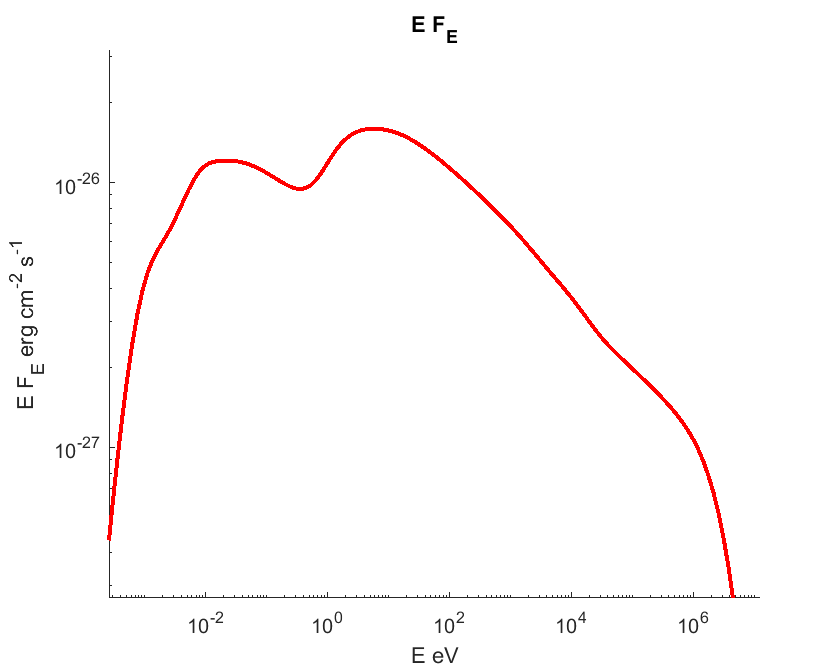
\includegraphics[width=12.5 cm]{./fig/compton.png} 
	\caption{Энергетическая плотность потока синхротронного излучения от тестового источника}
	\label{compton}
\end{figure}

\subsection{Распад пионов}
\subsection{Тормозное излучение}

